Rather than calling it denoising, better word in image reconstruction because
Image Reconstruction:

Purpose: To reconstruct an image from incomplete, noisy, or indirect measurements. This is often used in medical imaging (e.g., MRI, CT scans), computational photography, and computer vision applications. 

Reconstruction involves generating a complete image from partial or indirect data, which can include denoising and deblurring as sub-tasks.

\section{Address reconstruction/denoising schemes}
VST with BM3D: BM3D uses collaborative filtering, which is also used in recommender systems [citation need]
PnP iterative stuff
maybe non local sometime
UNET noise2noise

\section{What is poisson}

\begin{figure}
    \centering
    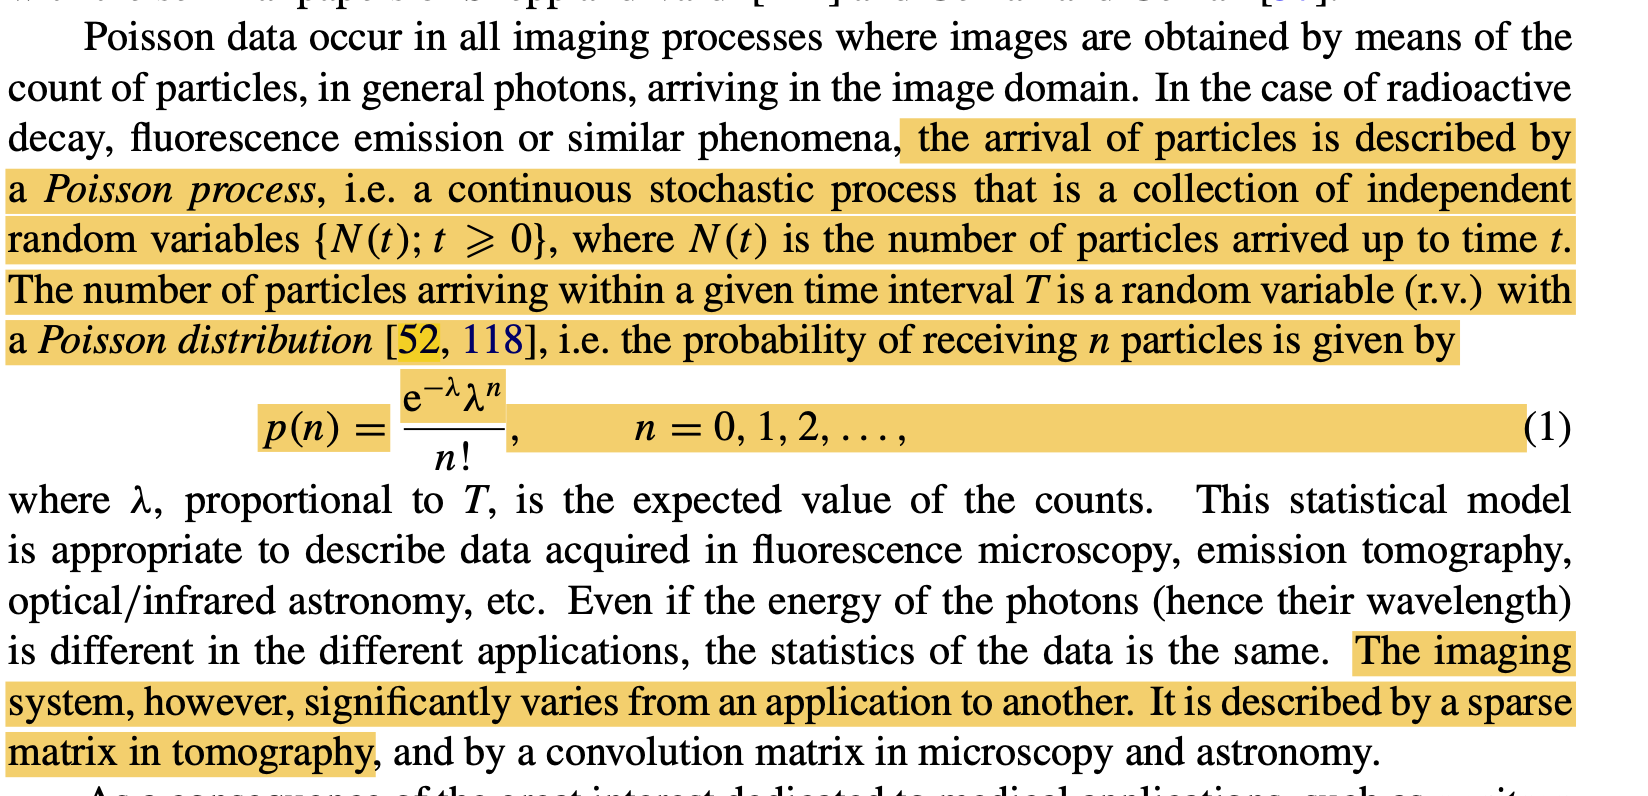
\includegraphics[width=1\linewidth]{images/JD-54-image.png}
    \caption{Enter Caption}
    \label{fig:enter-label}
\end{figure}

Taken from \cite{bertero_image_2009} which cites \cite{feller_introduction_1968}

\section{Comparsion of bm3d }
with and without anscombe on different datasets from flash, lab and fhi
Testing s

\section{Algorithms}

ERM 
Deep learning is just linear sepeartor problem with a non linear function applied to it like RELU